\documentclass{standalone}
\usepackage{pgfplots}
\usetikzlibrary{fillbetween}
\pgfplotsset{compat=1.7}

\begin{document}
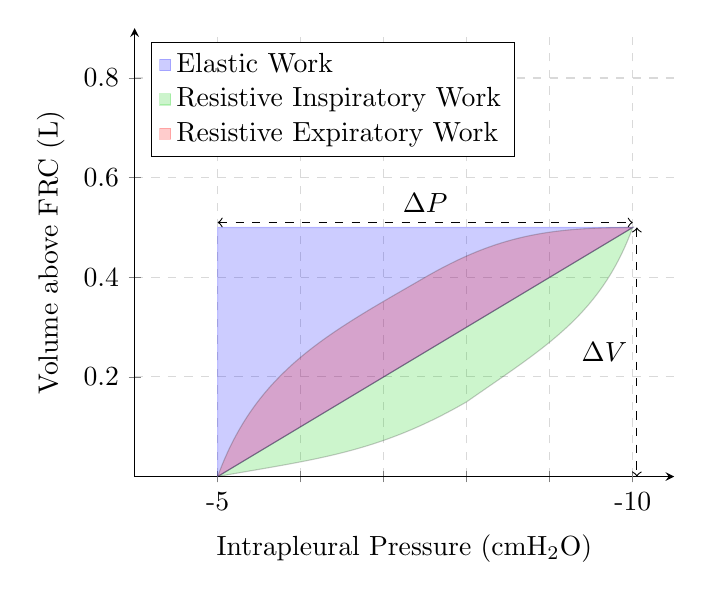
\begin{tikzpicture}
    \begin{axis}[
        axis x line=middle,
        axis y line=middle,
        grid = major,
        grid style={dashed, gray!30},
	  xticklabels={},
	extra x ticks={5, 10},
extra x tick labels = {-5, -10},
        xmin=4,
        xmax= 10.5,
        ymin= 0,
        ymax= 0.9,
	 ylabel near ticks,
	xlabel near ticks,
        xlabel=Intrapleural Pressure (cmH\textsubscript{2}O),
        ylabel=Volume above FRC (L),
clip=false,
legend pos = north west,
legend entries={Elastic Work, Resistive Inspiratory Work, Resistive Expiratory Work},
legend cell align={left}]

\draw[black, thin, dashed, <->] (axis cs: 10.05,0.5) -- node[left]{$\Delta V$} (axis cs: 10.05,0);
\draw[black, thin, dashed, <->] (axis cs: 5,0.51) -- node[above]{$\Delta P$} (axis cs: 10,0.51);

\draw[name=elastic, draw=blue, fill=blue, opacity=0.2]  (axis cs: 5,0) -- (axis cs: 10, 0.5)  -- (axis cs: 5,0.5) -- (axis cs: 5, 0);
\draw[name=insp, black, fill=green!80!black, opacity=0.2] (axis cs: 5,0) to[out=10, in=210] (axis cs: 8,0.15) to[out=35, in=-110] (axis cs: 10, 0.5) -- (axis cs: 5,0);
\draw[name=exp, black, fill=red, opacity=0.2] (axis cs: 5,0) to[out=70, in=210] (axis cs: 7.5,0.40)  to[out=30, in=180] (axis cs: 10, 0.5)  -- (axis cs: 5,0);



 \addlegendimage{blue, only marks, opacity=0.2, mark=square*}
 \addlegendimage{green!80!black, only marks, mark=square*,  opacity=0.2}
 \addlegendimage{red, only marks, mark=square*, opacity=0.2}
\end{axis}

\end{tikzpicture} 
\end{document}